% !TEX root = thesis.tex

\section{Social Signal Prediction in Haggling Scenes}
We regress the function defined in Equation~\ref{equation:F_ours} using the data \ref{equation:measurement} collected from our haggling sequences. To further constrain the problem we assume that the target person is the seller positioned on the left side of the buyer, and as input we use the social signals of buyer ($\mathbf{X}^1$) and the other seller ($\mathbf{X}^2$). Based on our social signal measurements, the input and output of the function is represented as the measurement types described in Eq.~\ref{equation:measurement}. For example,
\begin{equation}
\begin{gathered}
\mathbf{Y} = [ \mathbf{x}^0, \boldsymbol{\theta}^0, \boldsymbol{\phi}^0, \mathbf{J}^0, \mathbf{F}^0, \mathbf{H}^0, \mathbf{V}^0, \mathbf{S}^0 ]\\
\mathbf{X}^i = [ \mathbf{x}^i, \boldsymbol{\theta}^i, \boldsymbol{\phi}^i, \mathbf{J}^i, \mathbf{F}^i, \mathbf{H}^i, \mathbf{V}^i, \mathbf{S}^i ],
\end{gathered}
\end{equation}
where we use the superscript 0 to denote the social signals of the target subject (the output of social signal prediction). Directly considering or predicting these full spectrum social signals is challenging and hard to analyze. In our work, we introduce several sub-problems using baseline methods. 

% \begin{figure*}
% 	\centering
% 	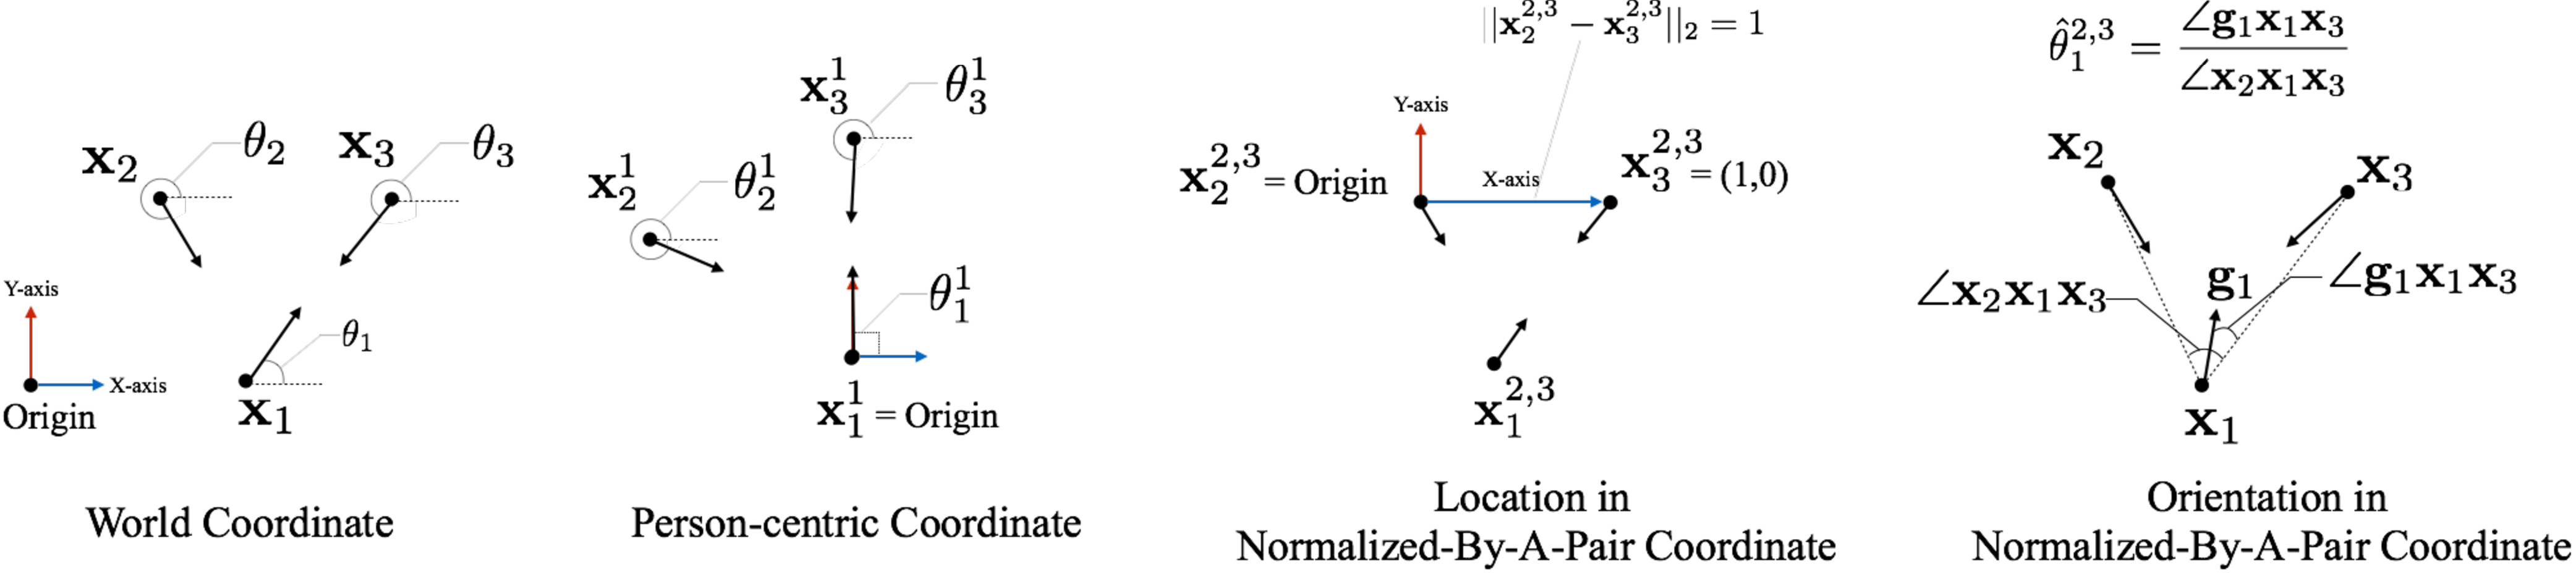
\includegraphics[width=\textwidth]{fig/ssp_notation3}
% 	\caption{Locations and orientations of an interacting group can be represented by different coordinate systems. (a) Locations and orientations in a world coordinate, (b) Locations and orientations in a person centric coordinate by person $\mathbf{P}_1$, (c) A location of $\mathbf{P}_1$  in a normalized coordinate by a pair of people $\mathbf{P}_2$ and $\mathbf{P}_3$, (d) An orientation of $\mathbf{P}_1$ in a normalized coordinate by a pair of people  $\mathbf{P}_2$ and $\mathbf{P}_3$. } 
% 	\label{fig:ssp_notation1}
% \end{figure*}

\subsection{Predicting Speaking}
As a simple task, we predict whether the target subject is currently speaking or not. This is a binary classification task and relatively easier to train compared to the task of regressing motion parameters as output. We first study the correlation between the speaking signal and the target person's own body motion, which should be more explicit. We then compare it with the performance of a classifier that uses the conversational partner's social signals. More specifically, a function $\mathcal{F}_{s0}$ uses the target person's own body motion $\mathbf{J}^0(t_0:t)$ to predict the speaking signal:
\begin{gather}	
\mathbf{S}^0(t) = \mathcal{F}_{s0} ( \mathbf{J}^0(t_0:t)),
\label{eq:speaking_0}
\end{gather}
and we compare this with a function $\mathcal{F}_{s12}$ that uses other subjects' body motions as input:
\begin{gather}	
\mathbf{S}^0(t) = \mathcal{F}_{s12} ( \mathbf{J}^1(t_0:t), \mathbf{J}^2(t_0:t)).
\label{eq:speaking_1}
\end{gather}
We hypothesize that the correlation between the speaking and body motion should be stronger than the speaking of the target and other people's body motions. But we still presume that there exists a clear correlation in building the function ~\ref{eq:speaking_1}; for example, if another person is talking we can guess the target person is not speaking due the ``turn-taking" implicitly followed during a social conversation. % This study is interesting because it demonstrates the existence of social correlation among social signals.

\subsection{Predicting Social Formations}
As another sub-problem, we predict the location and orientations of the target person. This problem is strongly related to Proxemics~\cite{Hall66} and F-formation~\cite{kendon90}, illustrating how humans use their space in social communications.
\begin{gather}	
 \mathbf{Y}_p (t_0:t) = \mathcal{F}_p ( \mathbf{X}_p^1(t_0:t), \mathbf{X}_p^2(t_0:t)),
 \label{eq:pred_formation}
\end{gather}
where $\mathbf{Y}_p$ and $\mathbf{X}_p^i$ contains global location and orientation signals $[\mathbf{x}, \boldsymbol{\theta}, \boldsymbol{\phi} ]$ for the target subject and others.
Note that we only consider the positions and orientations on the ground plane (in 2D), ignoring the height of the subjects. Thus $\mathbf{x} \in \mathbb{R}^2 $ representing $x$ and $z$ coordinate of the subjects. We use a 2D unit vector to represent the orientations $\theta \in \mathbb {R}^2$ and face orientation $\phi \in \mathbb{R}^2$, because the angle representation has a discontinuity issue when wrapping around $2\phi$ and $-2\phi$. In summary, $\mathbf{X}^i(t)$ and $\mathbf{X}^i(t)$ are a $6 \times N$ dimensional matrix where $N = t- t_0$ is the size of the temporal window. This prediction problem is intended to see whether the machine can learn how to build a social formation to interact with humans~\cite{vazquez2017towards}. Social formation is one of the most noticeable social properties with strong correlation, allowing us to easily evaluate the performance.


To implement this, we use a simple 1-D temporal convolutional neural network to model $\mathcal{F}_p$. The network is trained with a window of frames $N=120$ (corresponding to 4 seconds), but arbitrary length of input can be used in testing time since our network is fully convolutional. We use a simple encoder-decoder network. The encoder has  3 convolutional layers followed by dropout (0.25) and RELU, and 1D pooling layer (with stride 2). The decoder uses a single transposed convolution layer. We use L2 loss function with a L1 regularization term (with weight 0.1). We simply use the global position and orientations with standardization, rather than any local or relative coordinate.

\subsection{Predicting Kinesic Signals}
Predicting body motion in social situations (by using other subjects' signals) is challenging, because the correlation among body signals are subtle and less explicit. To study this, we present two baseline approaches here. 

\textbf{By Using Social Formation Only.} The first approach uses only the social formation information of other subjects:
\begin{gather}	
\mathbf{J}^0(t_0:t) = \mathcal{F}_{j0} ( \mathbf{X}_p^1(t_0:t), \mathbf{X}_p^2(t_0:t) ).
\end{gather}
This is an ill-posed problem with diverse possible solutions, because the formation signals of communication partners barely tells us about the detailed behavior of our target person. Yet, we can consider several required properties of the predicted skeleton. For example, the body location and orientation need to satisfy the social formation property, and when the target person's location is changing the appropriate leg motion needs to be predicted. Intuitively, we expect the predicted skeleton shows a similar social amount of information, location and orientations, as in social formation prediction, but using more complicated structure, body motion. In that sense, we can divide the function $\mathcal{F}_{j0}$ into two stages: predicting a social formation by $\mathcal{F}_p$ described in Eq.~\ref{eq:pred_formation} and predicting 3D body motion from the predicted social trajectory $\mathbf{Y}_p (t_0:t)$:
\begin{gather}	
 \mathbf{J}^0 (t_0:t) = \mathcal{F}_{p2J} \left(   \mathcal{F}_p \left( \mathbf{X}_p^1(t_0:t), \mathbf{X}_p^2(t_0:t) \right) \right) \nonumber \\ 
 = \mathcal{F}_{p2J} \left( \mathbf{Y}_p (t_0:t)  \right),
 \label{eq:pred_p2J}
\end{gather}
where $\mathcal{F}_{p2J}$ is a mapping between the target subject's own social trajectory to body skeleton. Since the trajectory (position and orientations) is a sub-part of the body behavior, we expect the predicted skeleton to contain similar signals as the social trajectory. For the function $\mathcal{F}_{p2b}$, we follow a similar approach to the work of Holden et al.~\cite{holden2016deep}. As in the Holden's work, we train an autoencoder to find the motion manifold space. As a major difference, we do not use foot step generator, and directly regress from the trajectory to the motion manifold space. We train this model in our dataset only, since the walking and running motion used in \cite{holden2016deep} is rare in our scenarios. 

\textbf{By using Body Motions as Input.} We can use the entire body signals of conversational partners as input for our function:
\begin{gather}	
\mathbf{J}^0 (t_0:t) = \mathcal{F}_{J2J} \left( \mathbf{J}^1 (t_0:t), \mathbf{J}^2 (t_0:t) \right) .
\end{gather}
In this particular example, we expect ``better" prediction quality than the previous baseline by using other subject's body motions as a cue to determine the target person's body motion. We found that this method shows more diverse upper body motion, responding the motions of other subjects. To this end, we present a hybrid method combining the upper body prediction results of this method to the root and leg motions of the previous method. 

% \subsection{Social Kinesic Signal Prediction: A Baseline}

% However, group discussion scenarios such our negotiation setting often do not have dominant location changes, and people make and keep a certain formation. But still a lot of nonverbal signals are transmitted by body gestures. To study this, as the next level of representation, we include full body landmarks,
% \begin{gather}	
% \mathbf{U}^i(t) = [\Delta \mathbf{x}^{i}_i(t), \Delta \theta_i(t),  \mathbf{j}_i(2:15,t)]^T
% \end{gather}
% where in this case the $\mathbf{x}^{i}_i(t)$ and $\theta_i(t)$ are computed from the root location (neck) of the body skeletons.

% As the richest version, we consider both body and face together:
% \begin{gather}	
% \mathbf{U}^i(t) = [\Delta \mathbf{x}^{i}_i(t), \Delta \theta_i(t),  \mathbf{j}_i(2:15,t), \mathbf{j}_i(k_f,t), \eta_i (t)]^T
% \end{gather}

% To study social communication, we consider the similar type of representation originated from other people. Let us assume that the target person $i$ receives signals from $j$-th person ($\mathbf{V}^j$). A way to represent the signals is by using exactly same representation as defined above.

% \begin{gather}	
% \mathbf{V}^j(t) = [\Delta \mathbf{x}^{j}_j(t), \Delta \theta_j(t)]^T\\ \nonumber
% \mathbf{V}^j(t) = [\Delta \mathbf{x}^{j}_j(t), \Delta \theta_j(t),  \mathbf{j}_j(2:15,t)]^T\\ \nonumber
% \mathbf{V}^j(t) = [\Delta \mathbf{x}^{j}_j(t), \Delta \theta_j(t),  \mathbf{j}_j(2:15,t), \mathbf{j}_j(k_f,t), \eta_j (t)]^T
% \end{gather}
% In this case, however, the formation information among people is completely ignored.

% As the second option, we can consider the representation of location differential of $j$-th person in our target person's coordination system, to relate them.
% \begin{gather}	
% \mathbf{V}^j(t) = [\Delta \mathbf{x}^{i}_j(t), \Delta \theta^i_j(t)]^T\\ \nonumber
% \mathbf{V}^j(t) = [\Delta \mathbf{x}^{i}_j(t), \Delta \theta^i_j(t),  \mathbf{j}_j(2:15,t)]^T\\ \nonumber
% \mathbf{V}^j(t) = [\Delta \mathbf{x}^{i}_j(t), \Delta \theta^i_j(t),  \mathbf{j}_j(2:15,t), \mathbf{j}_j(k_f,t), \eta_j (t)]^T
% \end{gather}
% In this case, relative formation information is implied in the differential of root locations.

% As the third option, we can consider relative formation from the target person without using differentials.
% \begin{gather}	
% \mathbf{V}^j(t) = [\mathbf{x}^{i}_j(t), \theta^i_j(t)]^T\\ \nonumber
% \mathbf{V}^j(t) = [\mathbf{x}^{i}_j(t), \theta^i_j(t),  \mathbf{j}_j(2:15,t)]^T\\ \nonumber
% \mathbf{V}^j(t) = [\mathbf{x}^{i}_j(t), \theta^i_j(t),  \mathbf{j}_j(2:15,t), \mathbf{j}_j(k_f,t), \eta_j (t)]^T
% \end{gather}


% \subsection{Social Kinesic Signal Prediction: Advanced}

% Actually modeling the body dymamics. Any noticable improvemenet?

% \section{Predicting Social Signals}
    
% Our model takes, as input, nonverbal signals from fixed window of time, and predicts future motion signals at a future time. We try multiple baselines and compare their social signal prediction performance. As defined in Equation~\ref{equation:F_ours}, the input is the combination of $\mathbf{U} (t-w:t)$ and $\mathbf{V} (t-w:t)$. $\mathbf{U}(t-w:t) \in \mathbf{R}^{N \times w}$  is a matrix where $N$ is the dimension of the chosen signals. To model social signals from other people together, we concatenate $U$ and $V$s vertically. For example, in our triadic negotiation cases, the input becomes,
% \begin{equation}
% \Theta(t) = [\mathbf{U}(t-w:t); \mathbf{V}^1  (t-w:t); \mathbf{V}^2  (t-w:t) ]
% \label{eq:input}
% \end{equation}
% , where $\mathbf{V}^1$ and $\mathbf{V}^2$ are signals from two other people. 

% To this end, we generate a training set from the following form,
% \begin{equation}
% \mathcal{F} ( \Theta(t) ) = \mathbf{U}(t+h).
% \end{equation}


% \subsection{Social Signal Prediction for Individuals}


% \subsection{Social Signal Prediction for Social Formation}


% \subsection{Social Signal Prediction for Kinesic Signals}

